\documentclass[11pt]{article}
%Gummi|065|=)
\title{\textbf{Meccano pentagons}}
\author{https://github.com/heptagons/meccano/penta}
\date{}

\usepackage{amsmath}
\usepackage[pdftex]{graphicx}
\usepackage{listings}
\usepackage{xcolor}
\definecolor{gray}{RGB}{245,245,245}

\lstset{
	backgroundcolor=\color{gray},
	frame=single,
	numbers=left,
	stepnumber=1,
	tabsize=2,
	basicstyle=\ttfamily\small,
	breaklines=true
}

\usepackage[margin=0.75in]{geometry}

% inkscape fig.svg --export-pdf=fig.pdf (prior version 1.0)

\usepackage{graphicx}
\begin{document}

\maketitle

\section{Meccano pentagons}

To identify a pentagon we use two angles $A$ and $B$. Some identities are solved for $a + b\sqrt{5}$ values to be used later.

\begin{align*}
5A &= {2\pi} \\
5B &= {\pi} \\
4\cos(A) &=  -1 + \sqrt{5} \\
4\cos(B) &=   1 + \sqrt{5} \\
8\cos^2(A) &= { 3 - \sqrt{5}} \\
8\cos^2(B) &= { 3 + \sqrt{5}} \\
4\cos(A)\cos(B) &= 1 \\
8\sin^2(A) &= 5 + \sqrt{5} \\
8\sin^2(B) &= 5 - \sqrt{5} \\
4\sin(A)\sin(B) &= \sqrt{5}
\end{align*}

\subsection{Pentagons of type 1}

\begin{figure}
\centering
\includegraphics[width=10cm]{figs/pentagon-type-1}
\caption{Meccano pentagon of type 1. From rods $a$, $b$ and $c$ with integer lengths we expect to find the rod $d$ length as integer too. Actually, the pentagon shown is the unique solved so far for small values of rods, $a=12$.}
\label{pentagon-type-1}
\end{figure}

A pentagon of type 1 is shown in figure \ref{pentagon-type-1}. We note three rods (or sections of rods) $a$, $b$, and $c$ at fixed angles and with integer sizes as it should be for any meccano figure. We want to find the fourth rod $d$ which also needs to be of integer size to make the pentagon.


We start by looking the rods' related formulas:

\begin{align*}
d_x^2 &= ( (a + c)\cos(A) + b)^2 \\
      &= (a + c)^2\cos^2(A) + 2(a + c)b\cos(A) + b^2 \\
d_y^2 &= ( (a - c)\sin(A))^2 \\
      &= (a - c)^2\sin^2(A) \\
d^2 &= d_x^2 + d_y^2 \\
    &= (a + c)^2\cos^2(A)
    + (a - c)^2\sin^2(A)
    + 2(a + c)b\cos(A)
    + b^2 \\
    &= (a + c)^2(3 - \sqrt{5})/8 \\
    &\qquad + (a - c)(5 + \sqrt{5})/8 \\
    &\qquad + 2(a + c)b(-1 + \sqrt{5})/4 \\
    &\qquad + b^2 \\
    &= m\sqrt{5} + n \\
\end{align*}

We define two variables $m$ and $n$. $m$ is the sum of all the terms multiplied by $\sqrt{5}$ while $n$ is the sum of all the terms not multipled by $\sqrt{5}$.

\begin{align*}
8m  &= -(a + c)^2 + (a - c)^2 + 4(a + c)b \\
    &= 4(a + c)b - 4ac \\
8n &= 3(a + c)^2 + 5(a - c)^2 - 4(a + c)b + 8b^2 \\
\end{align*}

Simplifying we get a value for the rod $d^2$ in function of the rest of rods.

\begin{align*}
m  &= \frac{ ab - ac + bc}{2} \\
n  &= a^2 + b^2 + c^2 - \frac{ ab + ac + bc }{2} \\
   &= a^2 + b^2 + c^2 - ac - m \\
d^2 &= m\sqrt{5} + a^2 + b^2 + c^2 - ac - m
\end{align*}

Now, we want rod $d$ to be as simple as possible so is good idea to make $m = 0$ wich requires $ac = (a + c)b$. This way the rod $d$ is a simpler function of $a$, $b$ and $c$.

\begin{align*}
ac &= (a + c)b \\
d &= \sqrt{ a^2 + b^2 + c^2 - ac }
\end{align*}

\subsubsection{Pentagon type 1 search}

With last equations, a program can iterate over the integer values of the rods $a$, $b$ and $c$ to discover the rod $d$ to be integer too. Next javascript program was run and found a single solution $a = 12, b = 3, c = 4, d = 11$ after 5000 iterations. Scaled solutions are discarded as repetitions.

\begin{lstlisting}
function meccano_pentagons_1(sols)
{
	this.find = (max)=> {
		for (let a=1; a < max; a++)
			for (let b=1; b <= max; b++)
				for (let c=0; c <= a; c++)
					if (a*c == (a + c)*b)
						mZero(a, b, c)
	}
	
	const mZero = (a, b, c)=> {
		const d = Math.sqrt(a*a + b*b + c*c - a*c)
		if (d > 0 && d % 1 === 0)
			dInteger(a, b, c, d)
	}

	const dInteger = (a, b, c, d) => {
		for (let i=0; i < sols.length; i++) {
			const s = sols[i]
			if (a % s.a == 0) {
				const f = a / s.a
				const bS = (b % s.b == 0) && b / s.b == f
				const cS = (c % s.c == 0) && c / s.c == f
				const dS = (d % s.d == 0) && d / s.d == f
				if (bS && cS && dS)
					return // scaled solution already
			}
		}
		sols.push({ a:a, b:b, c:c, d:d }) // solution!
	}
}
\end{lstlisting}

\subsubsection{Pentagons of type 1 results}

\begin{figure}
\centering
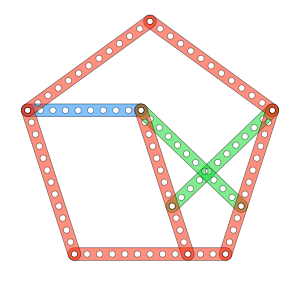
\includegraphics[width=7cm]{figs/pentagon-12a}
\caption{The smallest and maybe unique of pentagons of type 1. Is composed of 6 rods of
length 12 in color red, 2 rods of length 11 in green and 1 rod of size 9 in blue.}
\label{pentagon-12a}
\end{figure}

Figure \ref{pentagon-12a} shows the first pentagon of type 1 found.


\subsection{Pentagons of type 2}

\begin{figure}[htp]
\centering
\includegraphics[scale=1.00]{figs/pentagon-type-2.pdf}
\caption{Meccano pentagon of type 2. For rods $a$, $b$, $c$ and $d$ with integer lengths we expect
to find the rod $e$ with integer length too. Actually, the example shown is the smallest found $a=12, b=2, c=9, d=6, e=11$. For each solution there are two versions whether the green rods are used or the blue ones.}
\label{pentagon-type-2}
\end{figure}

A pentagon of type 2 is shown in figure \ref{pentagon-type-2}. We identify in this type of pentagon four rods $a$, $b$, $c$ and $d$ at fixed angles. We want to find a fifth rod $e$ with integer length to make the pentagon.

We start with the rods relation formulas

\begin{align*}
e_x &= b\cos(A) + a + c\cos(A) - d\cos(B) \\
      &= a + (b + c)\cos(A) - d\cos(B) \\
e_y &= c\sin(A) - b\sin(A) - d\sin(B) \\
      &= (c - b)\sin(A) - d\sin(B) 
\\
e^2 &= e_x^2 + e_y^2 \\
    &= a^2 + (b + c)^2\cos^2(A) + d^2\cos^2(B) \\
    &\qquad + 2a(b + c)\cos(A) - 2ad\cos(B) \\
    &\qquad - 2(b + c)d\cos(A)cos(B) \\
    &\qquad + (c - b)^2\sin^2(A) + d^2\sin^2(B) \\
    &\qquad - 2(c - b)d\sin(A)\sin(B) \\
    &= a^2 - 2(b + c)d / 4 \\
    &\qquad + (b + c)^2 ( 3 - \sqrt{5}) / 8 \\
    &\qquad + d^2       ( 3 + \sqrt{5}) / 8 \\
    &\qquad + 2a(b + c) (-1 + \sqrt{5}) / 4 \\
    &\qquad - 2ad( 1 + \sqrt{5}) / 4 \\
    &\qquad + (c - b)^2 ( 5 + \sqrt{5}) / 8 \\
    &\qquad + d^2       ( 5 - \sqrt{5}) / 8 \\
    &\qquad - 2(c - b)d ( \sqrt{5}) / 4 \\
    &= m\sqrt{5} + n \\
\end{align*}

As we did with the pentagon type 1, we define variables $m$ and $n$:

\begin{align*}
8m &= -(b+c)^2 + d^2 + 4a(b+c) - 4ad + (c-b)^2 - d^2 - 4(c-b)d \\
8n &= 8a^2 + 3(b+c)^2 + 3d^2 - 4a(b+c) - 4ad - 4(b+c)d + 5(c-b)^2 + 5d^2 \\
\end{align*}

Simplifying, we get a value for rod $e$ in function of the rest of rods:

\begin{align*}
m   &= \frac{(a - b)(c - d) + ab - cd}{2} \\
n   &= a^2 + b^2 + c^2 + d^2 - \frac{(a + b)(c + d) + ab + cd}{2} \\
    &=  a^2 + b^2 + c^2 + d^2 - ad - bc - cd - m \\
e^2 &= m\sqrt{5} + a^2 + b^2 + c^2 + d^2 - ad - bc - cd - m
\end{align*}

Again we decide to make $m = 0$ which now requires $cd = (a-b)(c-d)+ab$.
This way the rod $e$ is a simple function of rods $a$, $b$, $c$ and $d$:

\begin{align*}
cd &= (a - b)(c - d ) + ab \\
e &= \sqrt{a^2 + b^2 + c^2 + d^2 - ad - bc - cd}
\end{align*}

\subsubsection{Pentagon type 2 search}

With last equations, another program, for the pentagon type 2, can iterate over the integer values of rods $a$, $b$, $c$ and $d$ to discover a rod $e$ with integer length too. Next javascript program was run and found 40 different pentagons with rods length $<=$ 183.

\begin{lstlisting}
func pentagons_type_2(max int) {

	sols := make([][]int, 0)

	add := func(a, b, c, d, e int) {
		for _, s := range sols {
			if a % s[0] != 0 { continue }
			// new a is a factor of previous a
			f := a / s[0]
			if t := b % s[1] == 0 && b / s[1] == f; !t { continue }
			if t := c % s[2] == 0 && c / s[2] == f; !t { continue }
			if t := d % s[3] == 0 && d / s[3] == f; !t { continue }
			if t := e % s[4] == 0 && e / s[4] == f; !t { continue	}
			return // scaled solution already found (reject)
		}
		// solution!
		sols = append(sols, []int{ a, b, c, d, e })
		fmt.Printf("%3d a=%3d b=%3d c=%3d d=%3d e=%3d\n", len(sols), a, b, c, d, e)
	}

	check := func(a, b, c, d int) {
		f := float64(a*a + b*b + c*c + d*d - a*d - b*c - c*d)
	    if f < 0 {
	    	return
	    }
		if e := int(math.Sqrt(f)); math.Pow(float64(e), 2) == f {
			add(a, b, c, d, e)
		}
	}

    for a := 1 ; a < max; a++ {
    	for b := 1; b < a; b++ {
        	for c := 1; c < a; c++ {
          		for d := 1; d < a; d++ {
            		if ((a - b)*(c - d) + a*b == c*d) {
              			check(a, b, c, d)
              		}
              	}
            }
        }
    }
}
\end{lstlisting}

\subsection{Type 2 results}
The program found as much as 124 pentagons of type 2 for $a <= 488$.

\begin{lstlisting}
  1 a= 12 b=  2 c=  9 d=  6 e= 11
  2 a= 12 b=  6 c=  3 d= 10 e= 11
  3 a= 31 b=  4 c= 28 d= 16 e= 31
  4 a= 31 b= 15 c=  3 d= 27 e= 31
  5 a= 38 b= 12 c= 18 d= 21 e= 31
  6 a= 38 b= 17 c= 20 d= 26 e= 31
  7 a= 48 b=  8 c= 24 d= 21 e= 41
  8 a= 48 b= 12 c=  9 d= 20 e= 41
  9 a= 48 b= 27 c= 24 d= 40 e= 41
 10 a= 48 b= 28 c= 39 d= 36 e= 41
 11 a= 72 b= 21 c= 48 d= 40 e= 61
 12 a= 72 b= 24 c= 16 d= 39 e= 61
 13 a= 72 b= 32 c= 24 d= 51 e= 61
 14 a= 72 b= 33 c= 56 d= 48 e= 61
 15 a= 78 b= 27 c=  4 d= 42 e= 71
 16 a= 78 b= 36 c= 74 d= 51 e= 71
 . . .
119 a=488 b= 72 c= 15 d= 96 e=451
120 a=488 b=132 c=423 d=276 e=451
121 a=488 b=152 c=269 d=272 e=401
122 a=488 b=212 c= 65 d=356 e=451
123 a=488 b=216 c=219 d=336 e=401
124 a=488 b=392 c=473 d=416 e=451
\end{lstlisting}

Figures \ref{pentagons-2-31}, \ref{pentagons-2-38} and \ref{pentagons-2-48} show some of the pentagons of type 2 found.

\begin{figure}
\centering
\includegraphics[width=10cm]{figs/pentagons-2-31}
\caption{Pentagon of type 2 with $a=31$. This construction requires 7 rods of 
length 31 and 2 rods of length 27.}
\label{pentagons-2-31}
\end{figure}

\begin{figure}
\centering
\includegraphics[width=10cm]{figs/pentagons-2-38}
\caption{Pentagons of type 2 with $a=38$. Each construction requires 5 rods
of length 38, 2 rods of length 31 and 2 rods of length 26}
\label{pentagons-2-38}
\end{figure}

\begin{figure}
\centering
\includegraphics[width=15cm]{figs/pentagons-2-48}
\caption{Pentagons of type 2 with $a=48$}
\label{pentagons-2-48}
\end{figure}

\end{document}
